\chapter{Perfect Graphs and Structure}

In the preceding chapters, we saw that graph coloring, maximum clique, and maximum independent
set are NP-hard on general graphs. One cannot expect $\chi(G) = \omega(G)$ in general; indeed,
Mycielski's construction produces triangle-free graphs with arbitrarily high chromatic number.
This chapter studies a class where these problems become tractable: the \emph{perfect graphs},
where $\chi(H) = \omega(H)$ holds for every induced subgraph $H$. On perfect graphs, coloring,
maximum clique, maximum independent set, and minimum clique cover are all solvable in polynomial
time. We examine the structural characterizations of Berge and Lov\'asz, focus on chordal
graphs and their linear-time elimination orderings, and see how continuous convex relaxations
solve combinatorial problems.

\begin{historybox}
The concept of perfect graphs was born in information theory. In 1956, Claude Shannon
posed the fundamental problem of calculating the \emph{zero-error capacity} of a noisy
channel: transmitting symbols over a communications channel where certain pairs of signals
can be confused by receiver noise. Shannon proved that the maximum number of mutually
distinguishable single-letter messages is exactly the independence number $\alpha(\Gph)$
of the confusability graph.

In 1961, French mathematician Claude Berge observed that for several well-behaved graph
families --- bipartite graphs (K\H{o}nig 1931), interval graphs (Hajnal--Sur\'anyi 1958),
and comparability graphs of posets (Dilworth 1950) --- the chromatic number $\chi(H)$
consistently equaled the clique number $\omega(H)$ for every induced subgraph $H$.
Berge called these graphs \emph{perfect} and formulated two famous conjectures: the Weak
Perfect Graph Conjecture (a graph is perfect if and only if its complement is perfect) and
the Strong Perfect Graph Conjecture (a graph is perfect if and only if neither $G$ nor
$\overline{G}$ contains an induced odd cycle of length at least 5).

In 1972, 24-year-old Hungarian mathematician L{\'a}szl{\'o} Lov{\'a}sz proved the Weak
Conjecture using his Replication Lemma. Lov\'asz later introduced the semidefinite $\vartheta$
function, which Martin Gr{\"o}tschel, Lov{\'a}sz, and Alexander Schrijver (1981) optimized via
the ellipsoid method to give the first polynomial-time algorithms for coloring, clique, and
independent set on any perfect graph. The Strong Conjecture was finally proved in 2002
(published 2006) by Maria Chudnovsky, Neil Robertson, Paul Seymour, and Robin Thomas in a
landmark 178-page decomposition theorem. Polynomial-time recognition of perfect graphs
was established shortly after by Chudnovsky, G{\'e}rard Cornu{\'e}jols, Xinming Liu,
Seymour, and Kristina Vu{\v{s}}kovi{\'c} (2005). Today, finding a purely combinatorial
polynomial-time coloring algorithm for general perfect graphs that avoids semidefinite
programming remains a major open problem.
\end{historybox}

\chapterline

\section{What perfection means}

Start with two numbers attached to every graph $\Gph=(V,E)$.

\begin{definition}[Clique and chromatic numbers]\label{ch30:def-omega-chi}
The \emph{clique number} $\omega(\Gph)$ is the size of the largest set of pairwise-adjacent vertices. The \emph{chromatic number} $\chi(\Gph)$ is the fewest colors needed so that adjacent vertices get different colors.
\end{definition}

There is always a one-sided relationship between them.

\begin{proposition}[The trivial bound]\label{ch30:prop-trivial-bound}
For every graph $\Gph$, $\chi(\Gph)\ge\omega(\Gph)$.
\end{proposition}

\begin{proof}
A clique of size $\omega$ is a set of $\omega$ mutually adjacent vertices. In any proper coloring no two of them may share a color, so at least $\omega$ colors are spent on the clique alone. Hence any proper coloring uses $\ge\omega$ colors, and the minimum $\chi$ is $\ge\omega$.
\end{proof}

So $\omega$ is a \emph{lower bound} on $\chi$: you cannot color with fewer colors than the size of your biggest clique forces. The natural question is whether the clique is the \emph{only} obstruction. Sometimes it is not.

\begin{intuitionbox}
Think of $\omega(\Gph)$ as the ``obvious reason'' a graph needs many colors: a big clique simply cannot be squeezed into few color classes. The gap $\chi-\omega$ measures coloring difficulty that has \emph{no} local clique witness --- difficulty that comes from the global shape of the graph, like a long odd cycle that locally looks tree-like but globally refuses two colors. A \emph{perfect} graph is one with no such hidden difficulty anywhere: the obvious lower bound is always tight.
\end{intuitionbox}

The smallest example where the bound is loose is the $5$-cycle.

\begin{figure}[H]
\centering
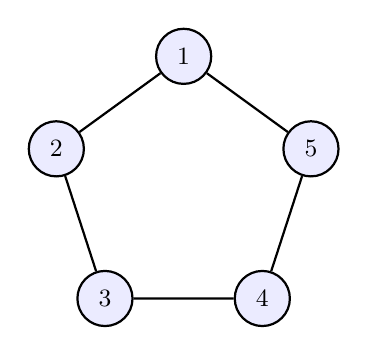
\begin{tikzpicture}[every node/.style={circle,draw,fill=blue!8,minimum size=7mm,inner sep=1pt,font=\small},thick]
  \foreach \i/\a in {1/90,2/162,3/234,4/306,5/18}{
    \node (\i) at (\a:1.7) {\i};
  }
  \draw (1)--(2)--(3)--(4)--(5)--(1);
\end{tikzpicture}
\caption{The cycle $C_5$. It has no triangle, so $\omega(C_5)=2$. But it has an odd number of vertices, so two colors fail: $\chi(C_5)=3$. The gap $\chi-\omega=1$ certifies that $C_5$ is \emph{not} perfect.}
\label{ch30:fig-c5}
\end{figure}

In $C_5$ the largest clique is a single edge, $\omega=2$. Yet you cannot $2$-color an odd cycle: walk around it alternating colors and you arrive back at the start needing the color you began with to differ from itself. So $\chi(C_5)=3>2=\omega(C_5)$. The trouble is global --- every local neighborhood is just a path --- which is exactly the kind of hidden difficulty perfection forbids.

Perfection asks for the bound to be tight not only on the whole graph but on every piece of it.

\begin{definition}[Perfect graph]\label{ch30:def-perfect}
A graph $\Gph$ is \emph{perfect} if $\chi(H)=\omega(H)$ for every induced subgraph $H\subseteq\Gph$ (including $H=\Gph$ itself).
\end{definition}

The induced-subgraph quantifier is essential and easy to underestimate. Requiring $\chi=\omega$ on the whole graph alone is a weak condition that many graphs satisfy by accident. Requiring it on \emph{every} induced subgraph is far more restrictive, and that restriction is what makes polynomial-time algorithms possible.

\begin{trapbox}
``$\chi(\Gph)=\omega(\Gph)$ for the whole graph'' does \emph{not} make $\Gph$ perfect. Consider $C_5$ together with a disjoint triangle $K_3$: the whole graph has $\omega=3$ and can be $3$-colored, so $\chi=\omega=3$ globally --- yet the induced $C_5$ still has $\chi=3>2=\omega$. The defect hides in a subgraph. Perfection is a hereditary property; you must check all induced subgraphs, and that is precisely why it is strong enough to be useful.
\end{trapbox}

\begin{focusbox}
Why should an algorithmist care about $\chi=\omega$ everywhere? Because it ties four separately-hard quantities together. We will see that on a perfect graph you can, in polynomial time, find:
\begin{itemize}
  \item a maximum clique (size $\omega$),
  \item a maximum independent set (size $\alpha$),
  \item an optimal coloring (using $\chi=\omega$ colors),
  \item a minimum clique cover (using $\bar\chi=\alpha$ cliques).
\end{itemize}
On a \emph{general} graph all four are $\mathrm{NP}$-hard. Perfection is the structural assumption that makes all four tractable.
\end{focusbox}

\section{The complement, and the Perfect Graph Theorem}

There is a symmetry hiding in Definition~\ref{ch30:def-perfect} that took two decades and a deep proof to confirm. Recall the \emph{complement} $\bar\Gph$: same vertices, and $uv$ is an edge of $\bar\Gph$ exactly when it is \emph{not} an edge of $\Gph$.

Cliques and independent sets swap under complementation. A set of pairwise-adjacent vertices in $\Gph$ is a set of pairwise-\emph{non}-adjacent vertices in $\bar\Gph$, so
\[
  \omega(\Gph)=\alpha(\bar\Gph),\qquad \alpha(\Gph)=\omega(\bar\Gph).
\]
Coloring swaps too, into something less familiar. A proper coloring of $\bar\Gph$ partitions $V$ into independent sets of $\bar\Gph$, which are cliques of $\Gph$. So $\chi(\bar\Gph)$ is the minimum number of cliques of $\Gph$ needed to cover all vertices --- the \emph{clique-cover number} $\bar\chi(\Gph)$. Putting these together, ``$\chi=\omega$ on $\bar\Gph$'' reads, in the language of $\Gph$, as ``the minimum clique cover equals the maximum independent set,'' i.e.\ $\bar\chi(\Gph)=\alpha(\Gph)$.

\begin{intuitionbox}
Perfection of $\Gph$ is a statement about coloring versus cliques. Perfection of $\bar\Gph$ is a statement about covering by cliques versus independent sets. On the surface, they look like completely different conditions. Lov\'asz proved, surprisingly, that they are equivalent: $\Gph$ is perfect if and only if $\bar\Gph$ is.
\end{intuitionbox}

\begin{theorem}[Perfect Graph Theorem; Lov\'asz 1972]\label{ch30:thm-pgt}
A graph $\Gph$ is perfect if and only if its complement $\bar\Gph$ is perfect.
\end{theorem}

We will not need the full machinery of $\vartheta$, but Theorem~\ref{ch30:thm-pgt} has a self-contained proof through a single lemma. The lemma says you may freely \emph{duplicate} a vertex and the result is still perfect.

\begin{definition}[Vertex replication]\label{ch30:def-replication}
To \emph{replicate} a vertex $v$ of $\Gph$, add a new vertex $v'$ adjacent to $v$ and to all neighbors of $v$ (so $v,v'$ are ``twins'' joined by an edge). Replicating with $k$ copies means doing this $k-1$ times, producing a clique $\{v=v_1,\dots,v_k\}$ all sharing $v$'s outside neighborhood.
\end{definition}

\begin{lemma}[Replication Lemma]\label{ch30:lem-replication}
If $\Gph$ is perfect and $\Gph'$ is obtained from $\Gph$ by replicating a vertex, then $\Gph'$ is perfect.
\end{lemma}

\begin{proof}
Induced subgraphs of $\Gph'$ are induced subgraphs of $\Gph$ or single replications of them, so by induction it suffices to show $\chi(\Gph')=\omega(\Gph')$ for one new twin $v'$ of $v$. Write $\omega=\omega(\Gph)$ and fix an $\omega$-coloring of $\Gph$.

\emph{Case 1: $v$ lies in some maximum clique $K$.} Then $K\cup\{v'\}$ is a clique, so $\omega(\Gph')=\omega+1$. Keep the coloring of $\Gph$ and give $v'$ one fresh color.

\emph{Case 2: $v$ lies in no maximum clique.} Then no clique through $v'$ exceeds $\omega$, so $\omega(\Gph')=\omega$. Let $C$ be the color class of $v$. Every maximum clique uses all $\omega$ colors, so it meets $C$, and not at $v$, so it meets $C\setminus\{v\}$. Hence $H=\Gph-(C\setminus\{v\})$ has $\omega(H)\le\omega-1$, and since $H$ is perfect it has an $(\omega-1)$-coloring. No vertex of $C\setminus\{v\}$ is adjacent to $v$ (they share a color), so none is adjacent to its twin $v'$, and $(C\setminus\{v\})\cup\{v'\}$ is independent. Give it the $\omega$-th color. That colors $\Gph'$ with $\omega$ colors.
\end{proof}

\begin{proof}[Proof of Theorem~\ref{ch30:thm-pgt}]
By symmetry it suffices to show: $\Gph$ perfect $\implies\bar\Gph$ perfect. Since induced subgraphs of a perfect graph are perfect, it is enough to show that every perfect $\Gph$ satisfies $\chi(\bar\Gph)=\omega(\bar\Gph)$, i.e.\ that $V$ can be covered by $\alpha=\alpha(\Gph)$ cliques of $\Gph$.

\emph{Key claim: some clique of $\Gph$ meets every maximum independent set.} Suppose not. Then each clique $K$ is missed by some maximum independent set $A_K$. Replicate each vertex $v$ into $t_v$ copies, where $t_v$ is the number of cliques $K$ with $v\in A_K$ (a vertex with $t_v=0$ is deleted). The blown-up graph $\Gph^\ast$ is perfect by Lemma~\ref{ch30:lem-replication}. Count three quantities, writing $N$ for the number of cliques of $\Gph$:
\begin{itemize}
  \item $\abs{V(\Gph^\ast)}=\sum_v t_v=\sum_K\abs{A_K}=\alpha N$.
  \item $\alpha(\Gph^\ast)\le\alpha$, because copies of one vertex form a clique, so an independent set of $\Gph^\ast$ uses at most one copy per vertex of an independent set of $\Gph$.
  \item A clique of $\Gph^\ast$ comes from a clique $K'$ of $\Gph$ and has $\sum_{v\in K'}t_v=\sum_K\abs{K'\cap A_K}$ vertices. Each term is at most $1$, and the term $K=K'$ is $0$, so $\omega(\Gph^\ast)\le N-1$.
\end{itemize}
Then $\chi(\Gph^\ast)\ge\abs{V(\Gph^\ast)}/\alpha(\Gph^\ast)\ge N>\omega(\Gph^\ast)$, contradicting perfection of $\Gph^\ast$.

\emph{Finish by induction on $\abs V$.} Take a clique $K$ meeting every maximum independent set. Then $\alpha(\Gph-K)=\alpha-1$, and $\Gph-K$ is perfect, so by induction it is covered by $\alpha-1$ cliques. Adding $K$ covers $V$ with $\alpha$ cliques.
\end{proof}

\begin{whybox}
The key fact in the proof is that replication preserves perfection. Once you can blow each vertex up into a clique of any size, you can convert a hypothetical violation of $\bar\chi=\alpha$ into a counting impossibility: a perfect graph cannot have more vertices than $\omega\cdot\alpha$, but a clique cover that is too large would force exactly that. The complement symmetry of perfection thus comes down to the bound $\abs{V}\le\omega\cdot\alpha$ holding on every induced subgraph.
\end{whybox}

\subsection*{The Strong Perfect Graph Theorem}

Berge's deeper conjecture pins down \emph{exactly} which graphs are perfect, by forbidding two families of induced subgraphs.

\begin{definition}[Holes and antiholes]\label{ch30:def-holes}
An \emph{odd hole} is an induced cycle $C_{2k+1}$ with $2k+1\ge 5$. An \emph{odd antihole} is the complement of an odd hole, $\overline{C_{2k+1}}$ with $2k+1\ge5$. A graph with no odd hole and no odd antihole as an induced subgraph is called \emph{Berge}.
\end{definition}

Both families are imperfect for the reason $C_5$ was: an odd hole $C_{2k+1}$ has $\omega=2$ but $\chi=3$, and an odd antihole $\overline{C_{2k+1}}$ has $\omega=k$ but $\chi=k+1$. So no perfect graph can contain either. Berge conjectured the converse.

\begin{theorem}[Strong Perfect Graph Theorem; Chudnovsky--Robertson--Seymour--Thomas 2006]\label{ch30:thm-spgt}
A graph is perfect if and only if it is Berge: it contains no odd hole and no odd antihole as an induced subgraph.
\end{theorem}

\begin{connectionbox}
The Lov\'asz theta function $\vartheta(\Gph)$ connects perfect graphs to Chapters~31, 32, and~38. Defined by a semidefinite program, it sits between $\omega$ and $\chi$ of the complement: $\omega(\Gph)\le\vartheta(\bar\Gph)\le\chi(\Gph)$. The Gr\"otschel--Lov\'asz--Schrijver algorithm computes $\vartheta$ via the ellipsoid method, and on perfect graphs $\vartheta(\bar\Gph)=\omega(\Gph)=\chi(\Gph)$ exactly. This is a rare case where a polynomial-time algorithm for an exact combinatorial invariant runs \emph{through} continuous optimization rather than around it. The combinatorial algorithms in the rest of this chapter avoid SDPs entirely --- but only for the structured subclasses, where elimination orderings replace the ellipsoid.
\end{connectionbox}

\section{Three structured families that are perfect}

The general perfect-graph algorithms are polynomial but heavy. Fortunately, the perfect graphs that arise in practice usually belong to a structured subclass with a fast combinatorial algorithm. Three families are the most common.

\begin{definition}[Interval graph]\label{ch30:def-interval}
$\Gph$ is an \emph{interval graph} if each vertex $v$ can be assigned a closed real interval $I_v$ so that $uv\in E$ iff $I_u\cap I_v\neq\emptyset$. The intervals are a \emph{representation} of $\Gph$.
\end{definition}

\begin{definition}[Comparability graph]\label{ch30:def-comparability}
$\Gph$ is a \emph{comparability graph} if its edges can be oriented transitively: there is an acyclic orientation such that whenever $u\to v$ and $v\to w$ are arcs, $u\to w$ is also an arc. Equivalently, $E$ is the comparability relation of some partial order on $V$.
\end{definition}

\begin{definition}[Chordal graph]\label{ch30:def-chordal}
$\Gph$ is \emph{chordal} (or triangulated) if every cycle of length $\ge 4$ has a \emph{chord}: an edge joining two vertices that are non-consecutive on the cycle. Equivalently, $\Gph$ has no induced cycle $C_k$ for any $k\ge4$.
\end{definition}

\begin{figure}[H]
\centering
\begin{tikzpicture}[font=\small]
  % interval representation
  \begin{scope}
    \node[anchor=east] at (-0.3,1.5) {\footnotesize intervals};
    \draw[very thick,sourceblue]   (0,1.5)--(2.0,1.5) node[right]{$a$};
    \draw[very thick,targetgreen]  (1.0,1.0)--(3.2,1.0) node[right]{$b$};
    \draw[very thick,quotientorange](2.6,0.5)--(4.4,0.5) node[right]{$c$};
    \draw[very thick,structurepurple](0.4,0.0)--(0.9,0.0) node[right]{$d$};
  \end{scope}
  % its interval graph
  \begin{scope}[xshift=6.2cm,yshift=0.4cm,every node/.style={circle,draw,fill=blue!8,minimum size=7mm,inner sep=1pt}]
    \node (a) at (0,1.4) {$a$};
    \node (b) at (1.6,1.4) {$b$};
    \node (c) at (1.6,0) {$c$};
    \node (d) at (0,0) {$d$};
    \draw (a)--(b); \draw (b)--(c); \draw (a)--(d);
  \end{scope}
\end{tikzpicture}
\caption{Left: four intervals on the line. $a$ overlaps $b$ and $d$; $b$ overlaps $a$ and $c$; $c$ overlaps $b$; $d$ overlaps $a$. Right: the resulting interval graph (a path $d$--$a$--$b$--$c$). Interval graphs are chordal, and chordal graphs are perfect.}
\label{ch30:fig-interval}
\end{figure}

These three families are not the same, but they nest and overlap in a way worth memorizing.

\begin{proposition}[Containments]\label{ch30:prop-containments}
Every interval graph is chordal. Every interval graph is also the complement of a comparability graph (a ``co-comparability'' graph). Every chordal graph and every comparability graph is perfect.
\end{proposition}

We prove the chordal case below, because the proof gives our main algorithm directly. The interval-implies-chordal direction is a quick exercise: a chordless cycle of length $\ge4$ among intervals cannot be realized on the line. The comparability-is-perfect direction follows from Mirsky's theorem (a longest chain equals the minimum antichain cover), an instance of Dilworth-type duality.

\begin{applicationbox}
Interval graphs model \emph{scheduling}: tasks occupy time intervals, two tasks conflict iff their intervals overlap, and a proper coloring with $\chi$ colors is an assignment of tasks to the fewest machines so that no machine runs two overlapping tasks. Because interval graphs are perfect, $\chi=\omega$: the number of machines you need equals the maximum number of tasks live at any single instant --- the obvious bound is achievable, and greedy by start time achieves it. Chordal graphs model \emph{sparse Gaussian elimination}: the ``fill-in'' you incur eliminating a symmetric matrix in a given order is exactly the set of edges you must add to make the graph chordal, and a perfect elimination ordering is a fill-free pivot order. Comparability graphs encode \emph{partial orders}: Dilworth's theorem (minimum chain cover $=$ maximum antichain) is the perfection statement for them.
\end{applicationbox}

\paragraph{A comparability graph, concretely.}
Take the partial order on $\{1,2,3,4,6,12\}$ given by divisibility: $x<y$ when $x$ divides $y$ and $x\neq y$. Its comparability graph joins two numbers iff one divides the other. A \emph{chain} (totally ordered subset) is a clique; an \emph{antichain} (pairwise incomparable subset) is an independent set. Here $\{1,2,4,12\}$ is a chain of length $4$, and $\{4,6\}$ is an antichain --- neither of $4$ and $6$ divides the other.

\begin{figure}[H]
\centering
\begin{tikzpicture}[every node/.style={circle,draw,fill=blue!8,minimum size=8mm,inner sep=1pt,font=\small},thick]
  \node (n1) at (0,0)    {$1$};
  \node (n2) at (-1.4,1.3) {$2$};
  \node (n3) at (1.4,1.3)  {$3$};
  \node (n4) at (-2.0,2.6) {$4$};
  \node (n6) at (0.4,2.6)  {$6$};
  \node (n12) at (-0.8,3.9){$12$};
  \draw (n1)--(n2); \draw (n1)--(n3);
  \draw (n2)--(n4); \draw (n2)--(n6); \draw (n3)--(n6);
  \draw (n4)--(n12); \draw (n6)--(n12);
  % transitive edges (lighter)
  \draw[edgegray] (n1) to[bend left=55] (n4);
  \draw[edgegray] (n1) to[bend right=55] (n6);
  \draw[edgegray] (n1) to[bend left=20] (n12);
  \draw[edgegray] (n2) to[bend left=30] (n12);
  \draw[edgegray] (n3) to[bend right=40] (n12);
\end{tikzpicture}
\caption{The divisibility order on $\{1,2,3,4,6,12\}$, drawn with cover edges dark and transitive comparabilities in gray. Every comparable pair is an edge of the comparability graph. The longest chain $1\mid2\mid4\mid12$ (or $1\mid2\mid6\mid12$, $1\mid3\mid6\mid12$) has length $4$, so $\omega=4$ and $\chi=4$; the largest antichain is $\{4,6\}$ (or $\{3,4\}$), so $\alpha=2$ and the minimum chain cover uses $2$ chains. Both equalities $\chi=\omega$ and $\bar\chi=\alpha$ hold --- the graph is perfect.}
\label{ch30:fig-divisibility}
\end{figure}

Mirsky's theorem says the height (longest chain) equals the minimum number of antichains needed to cover the order, which is the statement $\chi=\omega$ for the comparability graph. Dilworth's theorem is its dual: the width (largest antichain) equals the minimum number of chains needed to cover the order, which is $\bar\chi=\alpha$. The two dualities together are precisely perfection of the comparability graph and of its complement --- and by the Perfect Graph Theorem each implies the other.

\section{Chordal graphs: simplicial vertices and elimination orderings}

Chordal graphs are broad enough to include trees, interval graphs, and $k$-trees, yet structured enough that all four problems are solvable in linear time. The structure rests on one local notion.

\begin{definition}[Simplicial vertex]\label{ch30:def-simplicial}
A vertex $v$ is \emph{simplicial} if its neighborhood $N(v)$ is a clique --- every two neighbors of $v$ are adjacent. Equivalently, $v$ together with $N(v)$ forms a clique.
\end{definition}

\begin{figure}[H]
\centering
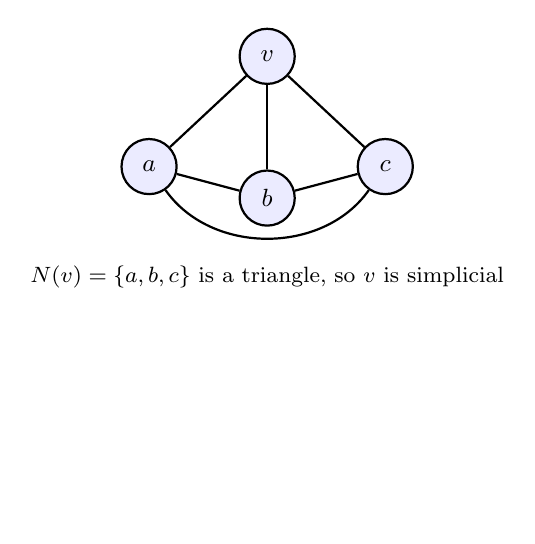
\begin{tikzpicture}[every node/.style={circle,draw,fill=blue!8,minimum size=7mm,inner sep=1pt,font=\small},thick]
  \node (v) at (0,0) {$v$};
  \node (a) at (-1.5,-1.4) {$a$};
  \node (b) at (0,-1.8) {$b$};
  \node (c) at (1.5,-1.4) {$c$};
  \draw (v)--(a); \draw (v)--(b); \draw (v)--(c);
  \draw (a)--(b); \draw (b)--(c); \draw (a) to[bend right=55] (c);
  \node[draw=none,fill=none,font=\footnotesize] at (0,-2.8) {$N(v)=\{a,b,c\}$ is a triangle, so $v$ is simplicial};
\end{tikzpicture}
\caption{A simplicial vertex $v$: its three neighbors are pairwise adjacent, so $\{v,a,b,c\}$ is a clique. Since $v$ lies inside a clique, it cannot be an interior vertex of any chordless cycle.}
\label{ch30:fig-simplicial}
\end{figure}

The reason simplicial vertices matter is a theorem of Dirac.

\begin{theorem}[Dirac 1961]\label{ch30:thm-dirac}
Every chordal graph with at least one vertex has a simplicial vertex. If the graph is not complete, it has \emph{two} non-adjacent simplicial vertices.
\end{theorem}

\begin{proof}
Induct on $\abs{V}$. A graph on one vertex is immediate, and a complete graph has every vertex simplicial. Let $\Gph$ be chordal and not complete, and pick two non-adjacent vertices $a,b$. Take a minimal vertex separator $S$ between them (a minimal set whose removal puts $a,b$ in different components). Let $A$ be the component of $\Gph-S$ containing $a$ and $B$ the one containing $b$.

First, $S$ is a clique. If two vertices $x,y\in S$ were non-adjacent, then by minimality of $S$ both $x$ and $y$ have a neighbor in $A$ and a neighbor in $B$; stitching a shortest $x$--$y$ path through $A$ with a shortest one through $B$ produces an induced cycle of length $\ge4$ with no chord, contradicting chordality.

Now apply the induction hypothesis to the chordal subgraph $\Gph[A\cup S]$. It has a simplicial vertex; if it is complete, any vertex of $A$ works, and otherwise it has two non-adjacent simplicial vertices, at least one of which lies in $A$ (since $S$ is a clique, the two cannot both lie in $S$). A vertex $v\in A$ that is simplicial in $\Gph[A\cup S]$ is simplicial in all of $\Gph$, because $v$'s only neighbors lie in $A\cup S$ --- none in $B$. Symmetrically $B$ yields a simplicial vertex of $\Gph$. The two lie in different components of $\Gph-S$, so they are non-adjacent.
\end{proof}

Dirac's theorem says you can always strip a chordal graph one simplicial vertex at a time. Record the stripping order and you get the central object of the chapter.

\begin{definition}[Perfect elimination ordering]\label{ch30:def-peo}
A \emph{perfect elimination ordering} (PEO) of $\Gph$ is an ordering $v_1,v_2,\dots,v_n$ of the vertices such that for each $i$, $v_i$ is simplicial in the subgraph induced on $\{v_i,v_{i+1},\dots,v_n\}$ --- that is, the \emph{later} neighbors of $v_i$ form a clique.
\end{definition}

\begin{theorem}[Fulkerson--Gross 1965]\label{ch30:thm-peo}
A graph is chordal if and only if it has a perfect elimination ordering.
\end{theorem}

\begin{proof}
($\Rightarrow$) If $\Gph$ is chordal, repeatedly apply Dirac's Theorem~\ref{ch30:thm-dirac}: pull out a simplicial vertex, call it $v_1$, and recurse on $\Gph-v_1$, which is again chordal (deleting a vertex cannot create a chordless cycle). The order of removal is a PEO by construction.

($\Leftarrow$) Suppose $\Gph$ has a PEO $v_1,\dots,v_n$ but, for contradiction, contains a chordless cycle $C$ of length $\ge4$. Let $v_i$ be the lowest-indexed vertex of $C$. Its two neighbors on $C$, call them $x$ and $y$, both come later in the order (they have higher index, since $v_i$ is lowest on $C$). They are both later-neighbors of $v_i$, so by the PEO property they must be adjacent. But $x$ and $y$ are non-consecutive on $C$ (they are the two neighbors of $v_i$, hence at distance $2$ on the cycle), so the edge $xy$ is a chord of $C$ --- contradicting that $C$ is chordless. Hence no such cycle exists and $\Gph$ is chordal.
\end{proof}

\begin{whybox}
A PEO turns ``no chordless cycle anywhere'' --- a global, hard-to-check condition --- into a \emph{local} elimination rule: process vertices in this fixed order, and at the moment you touch each one its surviving neighbors already form a clique. Every algorithm in this section is just ``walk the PEO and do something cheap at each vertex.'' The hard part is finding the order; once you have it, coloring, max-clique, and max-independent-set fall out in a single linear pass each.
\end{whybox}

\section{Finding a PEO in linear time: Lexicographic BFS}

How do we get the ordering? Dirac's proof gives an $\Oh(nm)$ method (repeatedly scan for a simplicial vertex). A much faster method is \emph{Lexicographic Breadth-First Search} (Lex-BFS) of Rose, Tarjan, and Lueker (1976), which produces a candidate ordering in $\Oh(n+m)$ time; a second linear pass verifies whether it is a genuine PEO and hence whether the graph is chordal.

\begin{intuitionbox}
Ordinary BFS breaks ties among the frontier arbitrarily. Lex-BFS breaks them with a rule: each unvisited vertex carries a \emph{label} listing which already-numbered vertices it is adjacent to, written in decreasing order of number. At each step pick the unvisited vertex whose label is lexicographically largest. Vertices adjacent to recently chosen, high-numbered vertices float to the front. The effect is to keep cliques together and visit a vertex right after its ``clique-mates,'' which is exactly what a (reversed) PEO needs.
\end{intuitionbox}

\begin{algorithm}[H]
\caption{Lex-BFS: produces an ordering $\sigma$ (a reversed-PEO candidate)}
\label{ch30:alg-lexbfs}
\KwIn{Graph $\Gph=(V,E)$ with $n$ vertices, $m$ edges.}
\KwOut{An ordering $\sigma(n),\sigma(n-1),\dots,\sigma(1)$ of $V$.}
Assign every vertex the empty label $\varepsilon$\;
\For{$i \leftarrow n$ \KwTo $1$}{
  Pick an unnumbered vertex $v$ of lexicographically \textbf{largest} label\;
  $\sigma(i)\leftarrow v$; mark $v$ numbered with number $i$\;
  \ForEach{unnumbered neighbor $w$ of $v$}{
    append $i$ to the label of $w$\;
  }
}
\Return $\sigma$\;
\end{algorithm}

Two implementation facts make this run in linear time. First, labels never need character-by-character comparison if you keep the unnumbered vertices in a \emph{partition refinement} structure: a doubly linked list of ``classes,'' each class being a set of vertices with identical labels so far, ordered by label. When vertex $v$ gets numbered, each class splits into (neighbors of $v$, non-neighbors), with the neighbor part promoted ahead. Each edge causes one split-membership move, so the total work is $\Oh(n+m)$. Second, the ordering Lex-BFS returns is a PEO --- when read in the elimination direction --- \emph{if and only if} the graph is chordal.

\begin{algorithm}[H]
\caption{Verify a PEO (and thus chordality) in linear time}
\label{ch30:alg-verifypeo}
\KwIn{Ordering $v_1,\dots,v_n$ (eliminate $v_1$ first), graph $\Gph$.}
\KwOut{\textsc{True} if it is a PEO, else a chordless-cycle witness.}
\For{$i\leftarrow 1$ \KwTo $n$}{$A(v_i)\leftarrow\emptyset$\;}
\For{$i\leftarrow 1$ \KwTo $n$}{
  Let $\mathrm{later}(v_i)=\{\,v_j : v_iv_j\in E,\ j>i\,\}$\;
  \If{$\mathrm{later}(v_i)\neq\emptyset$}{
    Let $u$ be the \textbf{earliest} (smallest index) vertex in $\mathrm{later}(v_i)$\;
    $A(u)\leftarrow A(u)\cup\big(\mathrm{later}(v_i)\setminus\{u\}\big)$\;
  }
  \If{$A(v_i)\not\subseteq \mathrm{later}(v_i)$}{
    \Return chordless cycle through $v_i$ (a required neighbor is missing)\;
  }
}
\Return \textsc{True}\;
\end{algorithm}

The verification idea: for each $v_i$, its later-neighbors must be a clique. Rather than test all pairs (quadratic), pass the responsibility to the earliest later-neighbor $u$: we only need $u$ to be adjacent to all the \emph{other} later-neighbors of $v_i$. Accumulating these requirements in $A(u)$ and checking, when we reach $u$, that $A(u)$ really sits inside $u$'s later-neighbors gives an $\Oh(n+m)$ test. Checking only $u$ is enough: the other later-neighbors of $v_i$ are then later-neighbors of $u$, and $u$'s own later-neighbors are verified to form a clique when $u$ is processed (induction from the right end of the order), so all of $\mathrm{later}(v_i)$ is a clique. If every check passes, the ordering is a PEO and $\Gph$ is chordal; the first failure exhibits two later-neighbors of some $v_i$ that are non-adjacent, which expands to an induced $C_4$ or longer.

\begin{labbox}
Run Lex-BFS on the graph in Figure~\ref{ch30:fig-tracegraph} below by hand. Keep the partition of unnumbered vertices as an ordered list of classes. At each step you should see one class split into the neighbors and non-neighbors of the vertex you just numbered. Stop when you have all six numbers, then read off the elimination order and check that each vertex's later-neighbors really do form a clique. The order you get should match the trace in Table~\ref{ch30:tab-trace}.
\end{labbox}

\begin{whybox}
The partition-refinement structure is worth a second look, because it is the reason the whole chapter runs in linear time rather than quadratic. Picture the unnumbered vertices as a left-to-right sequence of \emph{classes}, every vertex in a class sharing the same label so far, and classes ordered by label from large (left) to small (right). Numbering a vertex $v$ does exactly one thing to this sequence: it walks $v$'s adjacency list and, for every class that contains a neighbor of $v$, splits that class into its neighbor part and non-neighbor part, sliding the neighbor part one notch to the left (toward the larger labels). A vertex moves only when an incident edge is processed, and each edge is processed once, so the splits cost $\Oh(m)$ in total; the $n$ pick-and-remove steps cost $\Oh(n)$. No label is ever compared symbol by symbol --- the ordering of classes \emph{is} the lexicographic order, maintained incrementally. In short, ``compare strings'' is replaced by ``keep buckets sorted as you go.''
\end{whybox}

\section{A worked chordal graph, by hand}

Here is a six-vertex chordal graph. We will find a PEO with Lex-BFS, then color it, find its maximum clique, and find a maximum independent set --- all from the single ordering.

\begin{figure}[H]
\centering
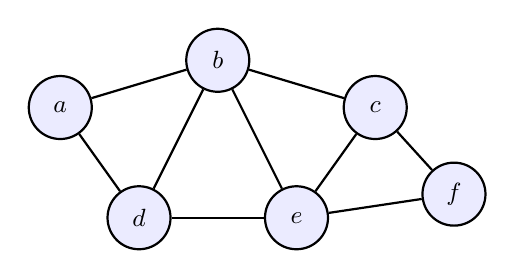
\begin{tikzpicture}[every node/.style={circle,draw,fill=blue!8,minimum size=8mm,inner sep=1pt,font=\small},thick]
  \node (a) at (0,2)   {$a$};
  \node (b) at (2,2.6) {$b$};
  \node (c) at (4,2)   {$c$};
  \node (d) at (1,0.6) {$d$};
  \node (e) at (3,0.6) {$e$};
  \node (f) at (5,0.9) {$f$};
  \draw (a)--(b); \draw (a)--(d); \draw (b)--(d);
  \draw (b)--(c); \draw (b)--(e); \draw (c)--(e);
  \draw (d)--(e); \draw (c)--(f); \draw (e)--(f);
\end{tikzpicture}
\caption{A chordal graph on six vertices. The triangles are $\{a,b,d\}$, $\{b,d,e\}$, $\{b,c,e\}$, $\{c,e,f\}$. There is no chordless cycle of length $\ge 4$: every such cycle here has a chord. Maximal cliques are the four triangles; $\omega=3$.}
\label{ch30:fig-tracegraph}
\end{figure}

\paragraph{Lex-BFS trace.}
We number from $6$ down to $1$ and break label ties by alphabetical order, starting from $a$. The label of a vertex records the numbers of its already-numbered neighbors, high-to-low.

\begin{table}[H]
\centering
\small
\begin{tabular}{c|c|l|c}
\toprule
step & numbered & labels of remaining (high-to-low) & ordered classes \\
\midrule
$6$ & $a\!=\!6$ & $b{:}6,\ d{:}6$; \ $c,e,f{:}\varepsilon$ & $\{b,d\}\,|\,\{c,e,f\}$ \\
$5$ & $b\!=\!5$ & $d{:}6,5$; \ $c{:}5,\ e{:}5$; \ $f{:}\varepsilon$ & $\{d\}\,|\,\{c,e\}\,|\,\{f\}$ \\
$4$ & $d\!=\!4$ & $e{:}5,4$; \ $c{:}5$; \ $f{:}\varepsilon$ & $\{e\}\,|\,\{c\}\,|\,\{f\}$ \\
$3$ & $e\!=\!3$ & $c{:}5,3$; \ $f{:}3$ & $\{c\}\,|\,\{f\}$ \\
$2$ & $c\!=\!2$ & $f{:}3,2$ & $\{f\}$ \\
$1$ & $f\!=\!1$ & --- & --- \\
\bottomrule
\end{tabular}
\caption{Lex-BFS on Figure~\ref{ch30:fig-tracegraph}. After numbering $a=6$, its neighbors $b,d$ get label ``$6$'' and jump ahead of $c,e,f$. Then $b=5$ (largest label, ties broken alphabetically among $\{b,d\}$). $d$'s label becomes ``$6,5$,'' beating $c,e$ (``$5$''). And so on. The numbering, high to low, is $a,b,d,e,c,f$.}
\label{ch30:tab-trace}
\end{table}

The \emph{elimination order} is the increasing-number order: $f(1), c(2), e(3), d(4), b(5), a(6)$. Equivalently, eliminate $f$ first, then $c$, $e$, $d$, $b$, $a$. Let us verify it is a PEO by checking later-neighbors (higher in elimination order $=$ later) form a clique.

\begin{table}[H]
\centering
\small
\begin{tabular}{c|c|l|c}
\toprule
vertex & elim.\ \# & later-neighbors & clique? \\
\midrule
$f$ & $1$ & $\{c,e\}$ & $ce\in E$? yes \checkmark \\
$c$ & $2$ & $\{e,b\}$ & $eb\in E$? yes \checkmark \\
$e$ & $3$ & $\{d,b\}$ & $db\in E$? yes \checkmark \\
$d$ & $4$ & $\{b,a\}$ & $ba\in E$? yes \checkmark \\
$b$ & $5$ & $\{a\}$ & singleton \checkmark \\
$a$ & $6$ & $\emptyset$ & \checkmark \\
\bottomrule
\end{tabular}
\caption{Every vertex's later-neighbors form a clique, so $f,c,e,d,b,a$ is a perfect elimination ordering. Theorem~\ref{ch30:thm-peo} confirms the graph is chordal.}
\label{ch30:tab-peocheck}
\end{table}

The four maximal cliques of this graph assemble into a \emph{clique tree}, the object that connects chordality to treewidth. Arrange the maximal cliques as tree nodes so that, for each vertex, the cliques containing it form a connected subtree (the running-intersection property). Here the tree is a single path.

\begin{figure}[H]
\centering
\begin{tikzpicture}[>=Stealth,
  cliquenode/.style={draw=structurepurple,rounded corners=2pt,fill=structurepurple!10,minimum height=8mm,inner sep=4pt,font=\footnotesize\bfseries},
  elnode/.style={circle,draw=sourceblue,fill=sourceblue!15,thick,minimum size=6.5mm,inner sep=0pt,font=\footnotesize\bfseries}
]
  % Lane 1: Clique Tree (Tree Decomposition)
  \node[font=\footnotesize\bfseries\scshape,text=structurepurple!80!black,anchor=west] at (-4.8,2.4) {Lane 1: Clique Tree (Maximal Cliques \& Separators)};
  \draw[gray!30,dashed] (-4.8,2.2) -- (4.8,2.2);

  \node[cliquenode] (k1) at (-3.6,1.4) {$\{a,b,d\}$};
  \node[cliquenode] (k2) at (-1.2,1.4) {$\{b,d,e\}$};
  \node[cliquenode] (k3) at (1.2,1.4)  {$\{b,c,e\}$};
  \node[cliquenode] (k4) at (3.6,1.4)  {$\{c,e,f\}$};

  \draw[very thick,structurepurple] (k1) -- node[midway,above,font=\tiny,fill=white,inner sep=1pt] {$\{b,d\}$} (k2);
  \draw[very thick,structurepurple] (k2) -- node[midway,above,font=\tiny,fill=white,inner sep=1pt] {$\{b,e\}$} (k3);
  \draw[very thick,structurepurple] (k3) -- node[midway,above,font=\tiny,fill=white,inner sep=1pt] {$\{c,e\}$} (k4);

  % Divider
  \draw[gray!40,thick] (-4.8,0.5) -- (4.8,0.5);

  % Lane 2: Elimination Tree
  \node[font=\footnotesize\bfseries\scshape,text=sourceblue!80!black,anchor=west] at (-4.8,0.1) {Lane 2: Elimination Tree (Parent = First Higher Neighbor in PEO)};
  \draw[gray!30,dashed] (-4.8,-0.1) -- (5.5,-0.1);

  % PEO order: f(1), c(2), e(3), d(4), b(5), a(6)
  \node[elnode] (ea) at (-3.5,-1.0) {$a_6$};
  \node[elnode] (eb) at (-2.1,-1.0) {$b_5$};
  \node[elnode] (ed) at (-0.7,-1.0) {$d_4$};
  \node[elnode] (ee) at (0.7,-1.0)  {$e_3$};
  \node[elnode] (ec) at (2.1,-1.0)  {$c_2$};
  \node[elnode] (ef) at (3.5,-1.0)  {$f_1$};

  \draw[<-,very thick,sourceblue] (ea) -- (eb);
  \draw[<-,very thick,sourceblue] (eb) -- (ed);
  \draw[<-,very thick,sourceblue] (ed) -- (ee);
  \draw[<-,very thick,sourceblue] (ee) -- (ec);
  \draw[<-,very thick,sourceblue] (ec) -- (ef);

  \node[font=\tiny,text=sourceblue!80!black] at (-3.5,-1.6) {PEO root ($a_6$)};
  \node[font=\tiny,text=sourceblue!80!black] at (3.5,-1.6) {Eliminated first ($f_1$)};
  \node[font=\tiny,edgegray] at (0,-2.05) {Assembly order: each node points to its first higher-ordered neighbor};
\end{tikzpicture}
\caption{Structural representations of the chordal graph. \textbf{Top (Lane~1):} The clique tree arranging the four maximal cliques into a tree decomposition of width $\omega-1=2$. Shared vertices on edges are minimal separators. \textbf{Bottom (Lane~2):} The elimination tree derived from the PEO $f(1), c(2), e(3), d(4), b(5), a(6)$, where each vertex directs an edge to its first higher-indexed neighbor. In Cholesky factorization, this tree captures all numerical dependencies without creating fill-in.}
\label{ch30:fig-cliquetree}
\end{figure}

\section{Linear-time coloring and maximum clique on a PEO}

With a PEO in hand, coloring is a one-pass greedy --- but applied in \emph{reverse} elimination order (eliminate-last vertex gets colored first), so that whenever we color a vertex its already-colored neighbors are exactly its later-neighbors, a clique.

\begin{algorithm}[H]
\caption{Optimal greedy coloring of a chordal graph from a PEO}
\label{ch30:alg-color}
\KwIn{Chordal $\Gph$, PEO $v_1,\dots,v_n$ (eliminate $v_1$ first).}
\KwOut{A proper coloring using exactly $\omega(\Gph)$ colors.}
\For{$i\leftarrow n$ \KwTo $1$}{
  $F\leftarrow\{\, \mathrm{color}(v_j) : v_iv_j\in E,\ j>i\,\}$ \tcp*{colors of already-colored (later) neighbors}
  $\mathrm{color}(v_i)\leftarrow$ smallest positive integer not in $F$\;
}
\Return $\mathrm{color}$\;
\end{algorithm}

\begin{theorem}[Chordal greedy is optimal]\label{ch30:thm-greedy-opt}
Algorithm~\ref{ch30:alg-color} produces a proper coloring with exactly $\omega(\Gph)$ colors, and the maximum color used equals the size of the largest clique. Hence for chordal graphs $\chi=\omega$ and both are found in $\Oh(n+m)$ time.
\end{theorem}

\begin{proof}
\emph{Properness} is immediate: when we color $v_i$ we avoid the colors of all neighbors already colored, and the neighbors colored later get colored avoiding $v_i$'s color in turn (each edge is resolved when its second endpoint is colored).

\emph{Color count.} Process in reverse elimination order. When $v_i$ is colored, its already-colored neighbors are precisely its later-neighbors $\mathrm{later}(v_i)$, which by the PEO property form a clique. Say $\abs{\mathrm{later}(v_i)}=k$. Those $k$ neighbors are pairwise adjacent and pairwise differently colored, so they occupy $k$ distinct colors; the greedy rule gives $v_i$ a color in $\{1,\dots,k+1\}$. Therefore $v_i$ receives color $\le k+1$, and the total number of colors used is at most $1+\max_i\abs{\mathrm{later}(v_i)}$.

Now $\{v_i\}\cup\mathrm{later}(v_i)$ is itself a clique of size $k+1$ (the later-neighbors are mutually adjacent and all adjacent to $v_i$). So $\max_i(\abs{\mathrm{later}(v_i)}+1)\le\omega(\Gph)$. Combining, the algorithm uses at most $\omega(\Gph)$ colors. By Proposition~\ref{ch30:prop-trivial-bound} it uses at least $\omega(\Gph)$. Hence exactly $\omega(\Gph)$, and $\chi=\omega$.

\emph{Max clique.} The largest clique is realized at the vertex $v_i$ maximizing $\abs{\mathrm{later}(v_i)}$: that vertex with its later-neighbors is a clique of size $\omega$, and no clique can be larger, since any clique's lowest-indexed vertex $v_j$ has the rest of the clique among its later-neighbors. So scanning the $\mathrm{later}$ sizes finds $\omega$ and an actual maximum clique. The running time is one pass with neighbor scans, $\Oh(n+m)$, given the PEO; Lex-BFS supplies the PEO in $\Oh(n+m)$.
\end{proof}

\paragraph{Coloring our example.}
Using the PEO $f,c,e,d,b,a$, we color in reverse: $a$ first, then $b,d,e,c,f$.

\begin{table}[H]
\centering
\small
\begin{tabular}{c|l|c}
\toprule
color step (reverse PEO) & already-colored later-neighbors and their colors & color chosen \\
\midrule
$a$ & none & $1$ \\
$b$ & $a{=}1$ & $2$ \\
$d$ & $a{=}1,\ b{=}2$ & $3$ \\
$e$ & $b{=}2,\ d{=}3$ & $1$ \\
$c$ & $b{=}2,\ e{=}1$ & $3$ \\
$f$ & $c{=}3,\ e{=}1$ & $2$ \\
\bottomrule
\end{tabular}
\caption{Greedy coloring along the reverse PEO. Colors used: $\{1,2,3\}$, so $\chi=3$. The largest $\mathrm{later}$-set had size $2$ (e.g.\ $d$ has later-neighbors $\{b,a\}$), giving clique $\{d,b,a\}$ of size $3=\omega$. Indeed $\chi=\omega=3$.}
\label{ch30:tab-color}
\end{table}

\begin{trapbox}
The reverse order matters. If you greedily color in the \emph{forward} elimination order ($f$ first), a vertex's already-colored neighbors are its \emph{earlier}-neighbors, which need not be a clique, and the bound $\le k+1$ fails --- greedy can then use more than $\omega$ colors even on a chordal graph. The PEO guarantees the clique property only for the \emph{later}-neighbors, so you must color last-eliminated first. A second classic slip: forgetting that the same Lex-BFS output, read forward versus backward, plays both roles --- it is the elimination order one way and the coloring order the other.
\end{trapbox}

\section{Maximum independent set and minimum clique cover on a PEO}

The independent-set problem is solved by a greedy that runs in the \emph{forward} elimination order. Take the first vertex of the PEO into the solution, delete it and all its neighbors, and repeat on what remains.

\begin{algorithm}[H]
\caption{Maximum independent set of a chordal graph from a PEO}
\label{ch30:alg-mis}
\KwIn{Chordal $\Gph$, PEO $v_1,\dots,v_n$ (eliminate $v_1$ first).}
\KwOut{A maximum independent set $S$ and a clique cover of equal size.}
$S\leftarrow\emptyset$; mark all vertices \textit{alive}\;
\For{$i\leftarrow 1$ \KwTo $n$}{
  \If{$v_i$ is alive}{
    $S\leftarrow S\cup\{v_i\}$\;
    Form clique $K_i\leftarrow\{v_i\}\cup\{\text{alive later-neighbors of }v_i\}$\;
    mark $v_i$ and all its alive neighbors \textit{dead} (assign them to cover-clique $K_i$)\;
  }
}
\Return $S$ and the cover $\{K_i\}$\;
\end{algorithm}

\begin{theorem}[Chordal MIS and clique cover]\label{ch30:thm-mis}
Algorithm~\ref{ch30:alg-mis} returns a maximum independent set $S$ and a clique cover using exactly $\abs{S}$ cliques. Hence on chordal graphs $\alpha=\bar\chi$, both computable in $\Oh(n+m)$.
\end{theorem}

\begin{proof}
\emph{$S$ is independent.} When $v_i$ is added we kill all its alive neighbors, so no two chosen vertices are adjacent.

\emph{The cover is valid and has size $\abs{S}$.} Each time we add $v_i$ to $S$ we create one clique $K_i=\{v_i\}\cup(\text{alive later-neighbors})$. Why is $K_i$ a clique? Because at the moment we pick $v_i$, its alive neighbors are all later-neighbors (the earlier ones were killed by previous picks), and by the PEO those form a clique. Every vertex is killed exactly once, assigned to the $K_i$ of the picked vertex that killed it, so the $K_i$ partition $V$ into $\abs{S}$ cliques.

\emph{Optimality, by duality.} We have produced an independent set $S$ and a clique cover $\mathcal{K}$ with $\abs{S}=\abs{\mathcal{K}}$. But \emph{any} independent set meets each clique at most once (two independent vertices cannot both sit in one clique), so $\alpha(\Gph)\le\bar\chi(\Gph)$ always. Our construction achieves $\abs{S}=\abs{\mathcal{K}}\ge\bar\chi\ge\alpha\ge\abs{S}$, forcing equality throughout: $S$ is maximum, $\mathcal{K}$ is minimum, and $\alpha=\bar\chi$. Each vertex is scanned once with a neighbor sweep, $\Oh(n+m)$.
\end{proof}

\begin{whybox}
The proof is a small duality argument, of the same form as max-flow/min-cut or LP duality. The ``primal'' object $S$ (an independent set) and the ``dual'' object $\mathcal{K}$ (a clique cover) satisfy a weak inequality $\abs{S}\le\abs{\mathcal{K}}$ for free, just from the meaning of the words. The greedy algorithm produces a matched pair, and a matched pair certifies that \emph{both} are optimal. This self-certifying property is what makes perfection useful algorithmically: a structured graph lets you build the optimum and its proof in the same pass.
\end{whybox}

\paragraph{Independent set on our example.}
PEO order $f,c,e,d,b,a$ (eliminate $f$ first).
\begin{itemize}
  \item $f$ alive $\Rightarrow$ take $f$. Kill $f$ and its neighbors $c,e$. Clique $K_f=\{f,c,e\}$. Alive: $d,b,a$.
  \item $c$ dead, skip. $e$ dead, skip.
  \item $d$ alive $\Rightarrow$ take $d$. Kill $d$ and its alive neighbors $b,a$. Clique $K_d=\{d,b,a\}$. Alive: none.
  \item $b,a$ dead, skip.
\end{itemize}
Result $S=\{f,d\}$, $\abs{S}=2=\alpha$. Clique cover $\{f,c,e\}$ and $\{d,b,a\}$, two cliques, $\bar\chi=2$. Check: $\{f,d\}$ is independent ($fd\notin E$), and you cannot find three pairwise non-adjacent vertices here, so $\alpha=2$. The duality $\alpha=\bar\chi=2$ holds (Figure~\ref{ch30:fig-peo-duals}).

\begin{figure}[H]
\centering
\begin{tikzpicture}[>=Stealth, every node/.style={font=\small},
  c1/.style={circle,draw=sourceblue,fill=sourceblue!18,very thick,minimum size=7mm,inner sep=0pt,font=\footnotesize\bfseries},
  c2/.style={circle,draw=targetgreen,fill=targetgreen!18,very thick,minimum size=7mm,inner sep=0pt,font=\footnotesize\bfseries},
  c3/.style={circle,draw=quotientorange,fill=quotientorange!20,very thick,minimum size=7mm,inner sep=0pt,font=\footnotesize\bfseries},
  isnode/.style={circle,draw=trapred,fill=trapred!20,very thick,minimum size=7.2mm,inner sep=0pt,font=\footnotesize\bfseries},
  vnode/.style={circle,draw=nodeblue,fill=blue!8,thick,minimum size=7mm,inner sep=0pt,font=\footnotesize}
]
  % Left panel: Reverse PEO Coloring & Max Clique
  \begin{scope}[xshift=-3.6cm]
    \node[font=\footnotesize\bfseries,text=sourceblue!85!black] at (2.1,3.3) {Reverse PEO ($a_6\to f_1$): $\chi = \omega = 3$};
    \node[c1] (a1) at (0,1.9)   {$a{:}1$};
    \node[c2] (b1) at (1.8,2.4) {$b{:}2$};
    \node[c3] (c1) at (3.6,1.9) {$c{:}3$};
    \node[c3] (d1) at (0.9,0.5) {$d{:}3$};
    \node[c1] (e1) at (2.7,0.5) {$e{:}1$};
    \node[c2] (f1) at (4.4,0.8) {$f{:}2$};
    \draw[thick,edgegray] (b1)--(c1) (b1)--(e1) (c1)--(e1) (d1)--(e1) (c1)--(f1) (e1)--(f1);
    \draw[line width=2pt,structurepurple] (a1)--(b1)--(d1)--(a1);
    \node[font=\scriptsize,align=center] at (2.1,-0.35) {3-coloring uses colors $\{1,2,3\}$\\[-1pt]\textcolor{structurepurple!85!black}{\textbf{Max clique}} $\{a,b,d\}$ certifies $\omega=3$};
  \end{scope}

  % Divider
  \draw[gray!35,dashed] (1.6,-0.7) -- (1.6,3.5);

  % Right panel: Forward PEO MIS & Clique Cover
  \begin{scope}[xshift=2.4cm]
    \node[font=\footnotesize\bfseries,text=trapred!85!black] at (2.1,3.3) {Forward PEO ($f_1\to a_6$): $\alpha = \bar\chi = 2$};
    \draw[rounded corners=8pt,draw=structurepurple!70,fill=structurepurple!8,dashed,thick] (-0.5,0.05) rectangle (2.25,2.9);
    \node[font=\scriptsize\bfseries,text=structurepurple!85!black] at (0.85,2.65) {$K_d=\{d,b,a\}$};
    \draw[rounded corners=8pt,draw=quotientorange!80!black,fill=quotientorange!8,dashed,thick] (2.3,0.05) rectangle (4.9,2.4);
    \node[font=\scriptsize\bfseries,text=quotientorange!85!black] at (3.6,2.15) {$K_f=\{f,c,e\}$};

    \node[vnode]  (a2) at (0,1.9)   {$a$};
    \node[vnode]  (b2) at (1.6,2.1) {$b$};
    \node[vnode]  (c2) at (3.5,1.6) {$c$};
    \node[isnode] (d2) at (0.8,0.6) {$d^\star$};
    \node[vnode]  (e2) at (2.8,0.55){$e$};
    \node[isnode] (f2) at (4.3,0.8) {$f^\star$};
    \draw[thick,edgegray] (a2)--(b2) (a2)--(d2) (b2)--(d2) (b2)--(c2) (b2)--(e2) (c2)--(e2) (d2)--(e2) (c2)--(f2) (e2)--(f2);
    \node[font=\scriptsize,align=center] at (2.1,-0.35) {\textcolor{trapred!85!black}{\textbf{Max indep.\ set}} $S=\{f^\star,d^\star\}$ ($\alpha=2$)\\[-1pt]covered by 2 cliques $K_f, K_d$ ($\bar\chi=2$)};
  \end{scope}
\end{tikzpicture}
\caption{Both dualities realized on the six-vertex chordal graph from a single PEO. \textbf{Left:} Coloring in reverse elimination order ($a_6\to f_1$) uses $\chi=3$ colors, matched by the purple $3$-clique $\{a,b,d\}$. \textbf{Right:} Sweeping in forward elimination order ($f_1\to a_6$) picks independent vertices $f^\star$ and $d^\star$ ($\alpha=2$) and partitions $V$ into their later-neighbor cliques $K_f=\{f,c,e\}$ and $K_d=\{d,b,a\}$ ($\bar\chi=2$).}
\label{ch30:fig-peo-duals}
\end{figure}

\begin{complexitybox}
On a chordal graph, given $\Gph$ by adjacency lists:
\begin{center}
\begin{tabular}{ll}
\toprule
task & time \\
\midrule
Find a PEO / decide chordality (Lex-BFS + verify) & $\Oh(n+m)$ \\
Optimal coloring ($\chi=\omega$ colors) & $\Oh(n+m)$ \\
Maximum clique (size $\omega$) & $\Oh(n+m)$ \\
Maximum independent set (size $\alpha$) & $\Oh(n+m)$ \\
Minimum clique cover (size $\bar\chi=\alpha$) & $\Oh(n+m)$ \\
\bottomrule
\end{tabular}
\end{center}
Every one of these is $\mathrm{NP}$-hard on a general graph. All of these rely on a single $\Oh(n+m)$ ordering. Interval graphs inherit all of this (they are chordal) and additionally admit an even simpler ``sort by left endpoint'' sweep for coloring.
\end{complexitybox}

\section{Why structure gives polynomial time}

The algorithmic pattern here recurs throughout the book.

\begin{aestheticbox}
The general optimization problems --- $\chi$, $\omega$, $\alpha$, $\bar\chi$ --- are $\mathrm{NP}$-hard because an arbitrary graph can encode arbitrary constraint satisfaction; there is no order to exploit. \emph{Perfection} is the promise that the simplest lower bound is always tight, which removes the gap that hardness hides in. \emph{Chordality} is a still stronger, purely combinatorial promise: the vertices can be linearly ordered so that each one is locally trivial (simplicial) at the moment it is processed. A linear order under which a global problem becomes a sequence of trivial local decisions is the recurring shape of efficient graph algorithms --- topological order for DAG dynamic programming, BFS layers for shortest paths, the PEO here, and tree-decomposition orders for bounded treewidth. Once the order is found, the algorithm is usually straightforward.
\end{aestheticbox}

\begin{connectionbox}
\textbf{What This Made Possible:}
Perfect graphs form a class on which four problems that are NP-hard in general
--- $\chi(\Gph)$, $\omega(\Gph)$, $\alpha(\Gph)$, and clique cover $\bar\chi(\Gph)$ --- become
solvable in polynomial time. On chordal and interval graphs, Lex-BFS and Perfect Elimination Orderings
yield optimal linear-time $\Oh(n+m)$ algorithms. On general perfect graphs, the
Gr{\"o}tschel--Lov{\'a}sz--Schrijver (1981) framework uses semidefinite programming and the
Lov{\'a}sz $\vartheta$ function to solve all four invariants in polynomial time. In addition,
a chordal graph's clique tree is a tree decomposition with width $\omega - 1$ and zero fill-in,
linking perfection directly to sparse Cholesky factorization and Gaussian elimination.

\textbf{Limitations:}
\begin{itemize}
  \item \emph{Extreme sensitivity to induced subgraphs:} Perfection requires $\chi(H) = \omega(H)$
        for \emph{every} induced subgraph. Adding or deleting a single edge that introduces an
        induced $C_5$ destroys perfection instantly, rendering the combinatorial guarantees void.
  \item \emph{Semidefinite programming overhead:} While chordal graphs admit fast $\Oh(n+m)$
        algorithms, computing $\chi$ or $\alpha$ on general non-chordal perfect graphs requires the
        ellipsoid method on the Lov{\'a}sz $\vartheta$ function, which is polynomial but of
        high degree and practically heavy.
\end{itemize}

\textbf{Where We Go Next:}
Lov{\'a}sz's work on perfect graphs showed that discrete graph
problems can be solved by continuous geometric relaxations and eigenvalues.
How do we translate a discrete graph into continuous physics and linear algebra?
In \textbf{Chapter~31 (The Graph Laplacian)}, we connect graphs to
continuous potential theory: representing edges as physical springs and matrices as
diffusion operators.
\end{connectionbox}

\begin{marginnotebox}
The hierarchy to keep in your head: \emph{trees} $\subset$ \emph{interval} $\subset$ \emph{chordal} $\subset$ \emph{perfect}, with \emph{bipartite} and \emph{comparability} graphs also sitting inside perfect by clean structural theorems. The Strong Perfect Graph Theorem says \emph{all} perfect graphs are exactly the Berge graphs (no odd hole, no odd antihole). For algorithms you almost always want the strongest structure you can prove your input has: chordality if you can get it (linear time), perfection as a fallback (polynomial via the Lov\'asz theta SDP).
\end{marginnotebox}

\section*{Exercises}
\addcontentsline{toc}{section}{Exercises}

\begin{exercise}[Imperfection certificates]
Show directly that the odd antihole $\overline{C_7}$ has $\omega=3$ and $\chi=4$, certifying it is not perfect. (Hint: a clique in $\overline{C_7}$ is an independent set in $C_7$; the largest is $3$. For $\chi$, a proper coloring of $\overline{C_7}$ is a partition of $C_7$ into cliques of $C_7$, i.e.\ edges and single vertices --- count how many you need to cover $7$ vertices.)
\end{exercise}

\begin{exercise}[The product bound]
Prove that for every perfect graph $\abs{V}\le\omega(\Gph)\cdot\alpha(\Gph)$, and show this can fail for imperfect graphs by exhibiting a graph with $\abs{V}>\omega\alpha$. (This inequality is the arithmetic core of the Perfect Graph Theorem; $C_5$ is the smallest counterexample on the imperfect side.)
\end{exercise}

\begin{exercise}[Replication, in full]
The proof of the Replication Lemma~\ref{ch30:lem-replication} handles one twin. Check its first step in full: every induced subgraph of $\Gph'$ is either an induced subgraph of $\Gph$ or a single replication of one. Then run both cases of the proof on $C_4$ with one vertex replicated, and conclude by induction that replicating any vertex any number of times preserves perfection.
\end{exercise}

\begin{exercise}[Interval $\Rightarrow$ chordal]
Prove that every interval graph is chordal. (Hint: suppose intervals realize a chordless cycle $v_1v_2\cdots v_k v_1$ with $k\ge4$. Consider the vertex whose interval has the leftmost right-endpoint and derive a contradiction from the cycle's non-adjacencies.)
\end{exercise}

\begin{exercise}[Trees are chordal, and more]
Show every tree is chordal and exhibit a PEO of a tree directly (no Lex-BFS): repeatedly remove a leaf. What are the maximal cliques of a tree, and what does Algorithm~\ref{ch30:alg-color} reduce to? Confirm $\chi=\omega=2$ for any tree with an edge.
\end{exercise}

\begin{exercise}[Break the forward greedy]
Find a chordal graph and a PEO for which coloring greedily in \emph{forward} elimination order (eliminate-first colored first) uses strictly more than $\omega$ colors. This shows the reverse-order requirement of Algorithm~\ref{ch30:alg-color} is essential, not a convenience.
\end{exercise}

\begin{exercise}[Lex-BFS by hand]
Run Lex-BFS on the $5$-cycle $C_5$ and on $C_5$ plus one chord. For each, write the elimination order it returns and run the PEO verifier (Algorithm~\ref{ch30:alg-verifypeo}). The verifier should fail on $C_5$ (not chordal); determine whether a single chord makes $C_5$ chordal, and confirm the verifier's verdict.
\end{exercise}

\begin{exercise}[Clique tree]
For the chordal graph of Figure~\ref{ch30:fig-tracegraph}, list the four maximal cliques and build a \emph{clique tree}: a tree whose nodes are the maximal cliques such that for every vertex $v$, the cliques containing $v$ form a connected subtree. Verify the ``running intersection'' property and explain why this tree is a tree decomposition of width $\omega-1=2$. (Figure~\ref{ch30:fig-cliquetree} shows one such tree; confirm it and decide whether any other clique tree exists here.)
\end{exercise}

\begin{exercise}[Comparability and Dilworth]
A comparability graph comes from a partial order $P$. State Dilworth's theorem (minimum chain cover $=$ maximum antichain) and explain why it is exactly the assertion $\bar\chi=\alpha$ for the comparability graph of $P$. Deduce, using the Perfect Graph Theorem~\ref{ch30:thm-pgt}, that comparability graphs are perfect.
\end{exercise}

\begin{exercise}[Recognizing interval graphs]
Sketch how to combine a chordality test with a check that the maximal cliques can be linearly ordered (the ``consecutive cliques'' property) to recognize interval graphs in polynomial time, and explain how a valid ordering of maximal cliques yields an interval representation. (Booth--Lueker's PQ-trees do this in linear time; you need only describe the high-level reduction.)
\end{exercise}

\begin{exercise}[Divisibility order]
For the divisibility comparability graph of Figure~\ref{ch30:fig-divisibility} on $\{1,2,3,4,6,12\}$, exhibit an optimal coloring with $\chi=\omega=4$ colors and a minimum chain cover with $\bar\chi=\alpha=2$ chains. Then extend the ground set to $\{1,2,\dots,12\}$ under divisibility, and compute $\omega$ (longest chain) and $\alpha$ (largest antichain) for the enlarged order. (Hint for $\alpha$: the integers in $\{7,8,\dots,12\}$ are pairwise non-dividing.)
\end{exercise}

\begin{exercise}[Partition refinement by hand]
Implement, on paper, the partition-refinement view of Lex-BFS: maintain the unnumbered vertices as an ordered list of classes and, at each numbering step, perform the neighbor/non-neighbor split described in the text. Run it on the graph of Figure~\ref{ch30:fig-tracegraph} and confirm you reproduce Table~\ref{ch30:tab-trace} class-by-class. Then argue that the total number of split operations over the whole run is $\Oh(m)$, so the algorithm is $\Oh(n+m)$.
\end{exercise}

\begin{exercise}[Perfection is not closed under everything]
Show that perfection is preserved by taking induced subgraphs and by complementation (the latter is Theorem~\ref{ch30:thm-pgt}), but is \emph{not} preserved by adding an arbitrary edge or by taking subgraphs that are not induced. Give a small concrete example for each failure. (Hint: a path $P_5$ is perfect; what single edge turns part of it into an induced $C_5$ inside a larger graph?)
\end{exercise}
